\begin{pastexam}[label={px:ntu-115-dsa-17}]{臺大資工所 115 學年度 第 17 題}
（單選）

(4 points) Consider the Binary Search Tree in Figure 1. If node 66 is removed (replacing it with its in-order successor), what is the resulting \textit{preorder} traversal sequence?
\begin{center}
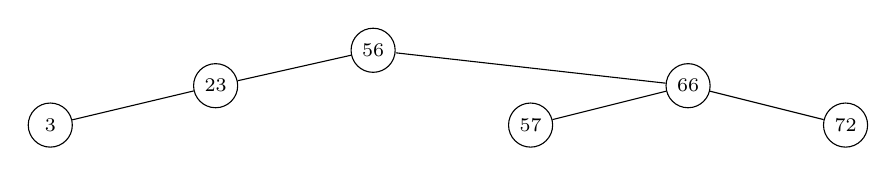
\begin{tikzpicture}[x=1cm,y=-1cm,
  every node/.style={circle,draw,inner sep=0pt,minimum size=5.6mm,font=\scriptsize}]
\node (n3) at (0,0.95) {3};
\node (n23) at (2.1,0.45) {23};
\node (n56) at (4.1,0) {56};
\node (n57) at (6.1,0.95) {57};
\node (n66) at (8.1,0.45) {66};
\node (n72) at (10.1,0.95) {72};
\draw (n56)--(n23) (n23)--(n3) (n56)--(n66) (n66)--(n57) (n66)--(n72);
\end{tikzpicture}\\[2pt]
Figure 1: Binary Search Tree
\end{center}
\begin{enumerate}[label=(\Alph*)]
\item 3, 23, 56, 57, 72.
\item 56, 23, 3, 72, 57.
\item 3, 23, 57, 72, 56.
\item 56, 23, 57, 72, 3.
\item None of the other choices.
\end{enumerate}
\end{pastexam}

\begin{pastsoln}
答案是 (B)。 圖中的樹寫成「鍵值(左,右)」是 $56(23(3,-),66(57,72))$。 $66$ 有兩個子節點，
屬於資結書第~9.2~節的情況 3。 中序後繼是右子樹 $\{72\}$ 的最小值 $72$，它沒有左子節
點，直接坐到 $66$ 的位置，接手左子樹 $57$，右邊是它原本的右子樹（空的）。 刪除之後是
$56(23(3,-),72(57,-))$。

前序走訪（先自己、再左、再右）：$56$，左子樹 $23, 3$，右子樹 $72, 57$，得到
$56, 23, 3, 72, 57$，就是 (B)。

其他選項：(A) 是中序走訪（BST 的中序一定由小到大，和刪除方式無關）。 (C) 是刪除之後的後序
走訪。 (D) 不是任何一種走訪：前序的最後一個應該是右子樹裡的節點，$3$ 卻在 $56$ 的左子樹。
(B) 正確，所以 (E) 不對。
\end{pastsoln}
